\documentclass{beamer}
\usepackage{../tut-slides}
\usepackage{../mathoperatorsAuD}

\usepackage{lmodern}
\usepackage{amsmath,amssymb}
\usepackage{wasysym}
\usepackage{stmaryrd}
\usepackage{enumerate}
%\usepackage[inline]{enumitem} 		%customize label
%\newcommand{\labelitemi}{\raisebox{1pt}{\scalebox{.9}{$\blacktriangleright$}}}
%\newcommand{\labelitemii}{$\vartriangleright$}
%\newcommand{\labelitemiii}{--}
\setbeamertemplate{itemize item}{\raisebox{1pt}{\scalebox{.9}{$\blacktriangleright$}}}
\setbeamertemplate{itemize subitem}{$\vartriangleright$}

\usepackage{booktabs}
\usepackage{tabularx}
\usepackage{tabu}
\newcommand*\head{\rowfont{\bfseries}}
\newcommand*{\tw}{\rowfont{\ttfamily}}
\renewcommand{\tabularxcolumn}[1]{>{\hspace{0pt}}m{#1}}
\usepackage{multirow}

\usepackage{tikz}
\usetikzlibrary{positioning}
\usepackage{cancel}

\usepackage{empheq}
\newcommand*\widefbox[1]{\fbox{\hspace{2em} #1 \hspace{2em}}}

\usepackage{tcolorbox}
\newtcolorbox{mymathbox}[1][]{colback=white, sharp corners, #1}

\usepackage{xcolor}
\usepackage{listings}
\lstset{numbers=left, 
	numberstyle=\tiny, 
	breaklines=true,
	backgroundcolor=\color{cdgray!20},
	numbersep=5pt,
	language=C,
	tabsize=2,
	basicstyle=\footnotesize\ttfamily,
	showstringspaces=false} 

\DeclareMathOperator{\ack}{\mathbf{ack}}
\usepackage{MnSymbol}

\newcommand{\col}[1]{\textcolor{cdpurple}{#1}}
\newcolumntype{R}[1]{>{\centering\arraybackslash}p{#1}}
\usepackage{tabularx}
\renewcommand{\tabularxcolumn}[1]{m{#1}}

\usepackage{qtree}
\usepackage[edges]{forest}

\newcommand{\lefttree}{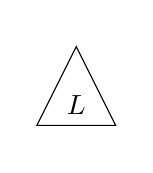
\begin{tikzpicture}
	\draw (0,0) node[anchor=north]{}
	-- (1,0) node[anchor=north]{}
	-- (.5,1) node[anchor=south]{}
	-- cycle;
	\draw (.5,.5) node[anchor=north]{$L$};
	\end{tikzpicture}}
\newcommand{\righttree}{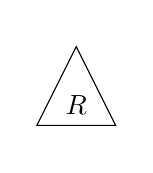
\begin{tikzpicture}
	\draw (0,0) node[anchor=north]{}
	-- (1,0) node[anchor=north]{}
	-- (.5,1) node[anchor=south]{}
	-- cycle;
	\draw (.5,.5) node[anchor=north]{$R$};
	\end{tikzpicture}}


\begin{document}	
	\title{Algorithmen und Datenstrukturen}
	\subtitle{Übung 10: AVL-Bäume \& Topologisches Sortieren}
	\author{Eric Kunze}
	\email{eric.kunze@mailbox.tu-dresden.de}
	\city{TU Dresden}
%	\institute{Lehrstuhl für Grundlagen der Programmierung}
	\titlegraphic{\includegraphics[width=2cm]{../TUD-white.pdf}}
	\date{15.01.2021}

	\maketitle


%%%%%%%%%%%%%%%%%%%%%%%%%%%%%%%%%%%%%%%%%%%%%%%%%%%%%%%%%%%%%%%%%%%%%%%%%%%%%


\section{AVL-Bäume}

\begin{frame} \frametitle{AVL-Bäume}
	Wir betrachten einen Baum $t$ und bezeichnen die \textit{Schlüssel} an den Knoten $n$ mit $s(n)$. 
	\pause
	
	\textbf{Suchbaum:} \Tree [.$s(n)$ [ .{\lefttree} ] [ .{\righttree} ] ] mit $L < s(n) < R$
	
	\pause
	
	Die \textit{Höhe} des Baumes bezeichnen wir mit $h(t)$.
	Wir ordnen jedem Knoten $n$ einen \textit{Balancefaktor} $b(n)$ zu:
	\begin{equation*}
		b(n) \defeq h(R) - h(L)
	\end{equation*}
	
	\pause
	\textbf{AVL-Baum:} Suchbaum mit $b(n) \in \menge{-1, 0, 1}$
\end{frame}

\begin{frame} \frametitle{Balancieren}
	\begin{itemize}
		\item Einfügen eines neuen Schlüssels $s$
		\item Berechne Balancefaktoren auf dem Pfad von $s$ zur Wurzel bis zum ersten Auftreten von $\pm 2$
		\pause
		\item \textbf{Balancierungsalgorithmus}: 
		\includegraphics[width=\linewidth]{./tut10_avl.jpg}
	\end{itemize}
\end{frame}

\begin{frame} \frametitle{Aufgabe 1}
	\begin{tabularx}{\linewidth}{m{2cm} m{.8cm} m{2cm} m{.8cm} m{2cm}}
		\begin{forest}
			[ $2$ [ $1$ ] [$3$ [,no edge, draw=none] [ $4$ ]  ] ] 
		\end{forest} 
		&
		$\overset{i(5)}{\longrightarrow}$
		&
		\begin{forest}
			[ $2^2$ [ $1$ ] [ $3^2$ [,no edge, draw=none] [ $4^1$ [,no edge, draw=none] [ $5^0$ ]  ] ]  ]
		\end{forest}  
		&
		$\overset{L(3)}{\longrightarrow}$
		&
		\begin{forest}
			[ $2$ [ $1$ ] [ $4$ [ $3$ ] [ $5$ ] ] ]
		\end{forest}
	\end{tabularx}
\end{frame}

\begin{frame} \frametitle{Aufgabe 1}
	\centering
	\begin{tabularx}{\linewidth}{m{2cm} m{.8cm} m{4cm}}
		\begin{forest}
			[ $4$ [ $2$ [,no edge, draw=none] [ $3$ ]  ] [ $5$ ] ]
		\end{forest}
		&
		$\overset{i(1)}{\longrightarrow}$
		&
		\begin{forest}
			[ $4^{-1}$ [ $2^0$ [ $1^0$ ] [ $3$ ]  ] [ $5$ ] ]
		\end{forest} 
	\end{tabularx}
\end{frame}

\begin{frame} \frametitle{Aufgabe 1}
	\footnotesize
	\begin{tabularx}{\linewidth}{m{4cm} m{.5cm} m{2.8cm}}
		\begin{forest}
			[ $8$ [ $5$ [ $3$ [ $2$ ] [ $4$ ]] [ $7$ [ $6$ ] [,no edge, draw=none]  ] ] [ $10$ [ $9$ ] [ $11$ ] ] ]
		\end{forest}
		&
		$\overset{i(1)}{\longrightarrow}$
		&
		\begin{forest}
			[ $8^{-2}$ [ $5^{-1}$ [ $3^{-1}$ [ $2^{-1}$ [ $1^0$ ] [,no edge, draw=none]] [ $4$ ]] [ $7$ [ $6$ ] [,no edge, draw=none]  ] ] [ $10$ [ $9$ ] [ $11$ ] ] ]
		\end{forest} 
		\\
		&
		$\overset{R(8)}{\longrightarrow}$
		&
		\begin{forest}
			[ $5$ [ $3$ [ $2$ [ $1$ ] [,no edge, draw=none] ] [ $4$ ] ] [ $8$ [ $7$ [ $6$ ] [,no edge, draw=none]] [ $10$ [ $9$ ] [ $11$ ]] ] ]
		\end{forest} 
	\end{tabularx}
\end{frame}

\begin{frame} \frametitle{Aufgabe 1}
	\small
	\begin{tabularx}{\linewidth}{m{2cm} m{.5cm} m{2.5cm} m{.5cm} m{2cm}}
		\begin{forest}
			[ $5$ [ $2$ [ $1$ ] [ $4$ ] ] [ $6$ ] ]
		\end{forest} 
		&
		$\overset{i(3)}{\longrightarrow}$
		&
		\begin{forest}
			[ $5^{-2}$ [ $2^{1}$ [ $1$ ] [ $4^{-1}$ [ $3^0$ ] [,no edge, draw=none]] ] [ $6$ ] ]
		\end{forest} 
		&
		$\overset{L(2)}{\longrightarrow}$
		&
		\begin{forest}
			[ $5$ [ $4$ [ $2$ [ $1$ ] [ $3$ ] ] [,no edge, draw=none] ] [ $6$ ] ]
		\end{forest}  \\ \\
		& $\overset{R(5)}{\longrightarrow}$
		& 
		\begin{forest}
			[ $4$ [ $2$ [ $1$ ] [ $3$ ]] [ $5$ [,no edge, draw=none] [ $6$ ] ] ]
		\end{forest}
	\end{tabularx}
\end{frame}


\section{Topologisches Sortieren}

\begin{frame} \frametitle{Topologisches Sortieren}
	\begin{itemize}
		\item Sortierung von \textit{Beziehungen} zwischen Objekten
		\item \textbf{Bsp.:} Ablauf eines Bauvorhabens \pause
		\begin{itemize}
			\item Baugrube ausheben (1) vor Fundament gießen (2)
			\item Fundament gießen (2) vor Wände setzen (3)
			\item $\dots$
			\item Elektrik im Bad (4) vor Fliesen (5)
			\item Wohnzimmer tapezieren (6) vor streichen (7)
			\item Wände streichen (5) und Fliesen (7) vor Möbel aufstellen (8)
		\end{itemize}
		\pause
		\begin{center}
			\includegraphics[width=0.7\linewidth]{tut10-topsort-bsp}
		\end{center}
		\pause
		\item In welcher Reihenfolge kann ich die Tätigkeiten abarbeiten?
	\end{itemize}
\end{frame}

\begin{frame} \frametitle{Topologisches Sortieren}
	\small
	Gegeben sei ein gerichteter, azyklischer Graph $G = (V,E)$. Eine \textbf{topologische Sortierung} von $G$ ist eine \textit{bijektive} Abbildung $\operatorname{ord} \colon V \to \menge{1, \dots, \card{V}}$, sodass für alle $v, v' \in V$ mit $(v,v') \in E$ die Relation
	$\operatorname{ord}(v) < \operatorname{ord}(v')$ gilt.
	
	\pause
	
	\textbf{Algorithmus:}
	
	\texttt{while} ( Elemente übrig ) \\
	\{  %\vspace{-\baselineskip}
		\begin{itemize}
			\item wähle Element $v$ ohne Vorgänger
			\item dekrementiere Anzahl der Vorgänger in den Nachfolgern von $v$
			\item füge $v$ der Ausgabeliste hinzu
			\item lösche $v$ aus $G$
		\end{itemize}
	\}
	 
\end{frame}

\begin{frame} \frametitle{Aufgabe 2}
	\textbf{Teil (a)}
	\begin{center}
		\includegraphics[width=0.5\linewidth]{tut10-aufgabe2a}
	\end{center}
	\pause
	Es gibt $4! \cdot 1! \cdot 3! = 24 \cdot 1 \cdot 6 = 144$ viele topologische Sortierungen.
\end{frame}

\begin{frame} \frametitle{Aufgabe 2}
	\textbf{Teil (b)}
	
	Es werden alle Möglichkeiten mit der $1$ am Anfang gestrichen, d.h. im ersten Block gibt es nur noch $4! - 3! = 24 - 6$ viele Möglichkeiten --- insgesamt also 
	\begin{equation*}
		(4! - 3!) \cdot 1! \cdot 3! = 18 \cdot 1 \cdot 6 = 108 \, .
	\end{equation*}

	\pause
	
	\textbf{Teil (c)}
	\begin{center}
		\includegraphics[width=0.7\linewidth]{tut10-aufgabe2c}
	\end{center}
\end{frame}

\end{document}